%Pakete;
%A4, Report, 12pt
\documentclass[ngerman,a4paper,12pt]{scrreprt}
\usepackage[a4paper, right=20mm, left=20mm,top=30mm, bottom=30mm, marginparsep=5mm, marginparwidth=5mm, headheight=7mm, headsep=15mm,footskip=15mm]{geometry}

%Papierausrichtungen
\usepackage{pdflscape}
\usepackage{lscape}

%Deutsche Umlaute, Schriftart, Deutsche Bezeichnungen
\usepackage[utf8]{inputenc}
\usepackage[T1]{fontenc}
\usepackage[ngerman]{babel}

%quellcode
\usepackage{listings}

%tabellen
\usepackage{tabularx}

%listen und aufzählungen
\usepackage{paralist}

%farben
\usepackage[svgnames,table,hyperref]{xcolor}

%symbole
\usepackage{latexsym,textcomp}
\usepackage{amssymb}

%font
\usepackage{helvet}
\renewcommand{\familydefault}{\sfdefault}

%Abkürzungsverzeichnisse
\usepackage[printonlyused]{acronym}

%Bilder
\usepackage{graphicx} %Bilder
\usepackage{float}	  %"Floating" Objects, Bilder, Tabellen...
\usepackage[space]{grffile} %Leerzechen Problem bei includegraphics
\usepackage{wallpaper} %Seitenhintergrund setzen
\usepackage{transparent} %Transparenz

%Tikz, Mindmaps, Trees
\usepackage{tikz}
\usetikzlibrary{mindmap,trees}
\usepackage{verbatim}

%for
\usepackage{forloop}
\usepackage{ifthen}

%Dokumenteigenschaften
\title{Summary CN1}
\author{Tobias Blaser}
\date{\today{}, Uster}


%Kopf- /Fusszeile
\usepackage{fancyhdr}
\usepackage{lastpage}

\pagestyle{fancy}
	\fancyhf{} %alle Kopf- und Fußzeilenfelder bereinigen
	\renewcommand{\headrulewidth}{0pt} %obere Trennlinie
	\fancyfoot[L]{\jobname} %Fusszeile links
	\fancyfoot[C]{Seite \thepage/\pageref{LastPage}} %Fusszeile mitte
	\fancyfoot[R]{\today{}} %Fusszeile rechts
	\renewcommand{\footrulewidth}{0.4pt} %untere Trennlinie

%Kopf-/ Fusszeile auf chapter page
\fancypagestyle{plain} {
	\fancyhf{} %alle Kopf- und Fußzeilenfelder bereinigen
	\renewcommand{\headrulewidth}{0pt} %obere Trennlinie
	\fancyfoot[L]{\jobname} %Fusszeile links
	\fancyfoot[C]{Seite \thepage/\pageref{LastPage}} %Fusszeile mitte
	\fancyfoot[R]{\today{}} %Fusszeile rechts
	\renewcommand{\footrulewidth}{0.4pt} %untere Trennlinie
}

\usepackage{changepage}

% Abkürzungen für Kapitel, Titel und Listen
%listen und aufzählungen
\usepackage{paralist}
\usepackage{mdwlist}

% list short cuts
\newcommand{\ul}{
	\begin{itemize}
}
\newcommand{\ulE}{
	\end{itemize}
}
\newcommand{\ol}{
	\begin{enumerate}
}
\newcommand{\olR}{
	\resume{enumerate}
}
\newcommand{\olE}{
	\end{enumerate}
}
\newcommand{\olS}{
	\suspend{enumerate}
}
\newcommand{\li}{
	\item
}
\newcommand{\dl}{
	\begin{description}
}
\newcommand{\di}[1]{
	\item[#1]
}
\newcommand{\dlE}{
	\end{description}
}
\newcommand{\ra}{
	$\rightarrow$
}

% chapter and section shortcuts
\newcommand{\ch}[1]{
	\chapter{#1}
}
\newcommand{\se}[1]{
	\section{#1}
}
\newcommand{\sse}[1]{
	\subsection{#1}
}
\newcommand{\sss}[1]{
	\subsubsection{#1}
}
\newcommand{\important}[1]{
	 \fcolorbox{black}{black}{ %
		\parbox{17cm}{%
			\vspace{0.1cm}
			\hspace{0.1cm}
   			\transparent{1.0}
			\color{white}
			\fontsize{12}{14} \selectfont #1
			\vspace{0.1cm}
   		}
    }
    \vspace{0.1cm}
}

\newcommand{\expl}[2]{
	 \fcolorbox{gray}{gray}{ %
		\parbox{17cm}{%
			\vspace{0.1cm}
			\hspace{0.1cm}
   			\transparent{1.0}
			\color{white}
			\fontsize{12}{14} \selectfont 
			\textbf{Erklärung #1:} #2
			\vspace{0.1cm}
   		}
    }
    \vspace{0.1cm}
}

\newcommand{\examp}[2]{
	 \fcolorbox{blue}{blue}{ %
		\parbox{17cm}{%
			\vspace{0.1cm}
			\hspace{0.1cm}
   			\transparent{1.0}
			\color{white}
			\fontsize{12}{14} \selectfont 
			\textbf{Beispiel (e) #1:} #2
			\vspace{0.1cm}
   		}
    }
    \vspace{0.1cm}
}

\newcommand{\exam}[1]{
	 \fcolorbox{orange}{orange}{ %
		\parbox{17cm}{%
			\vspace{0.1cm}
			\hspace{0.1cm}
   			\transparent{1.0}
			\color{white}
			\fontsize{12}{14} \selectfont 
			\textbf{Prüfung:} #1
			\vspace{0.1cm}
   		}
    }
    \vspace{0.1cm}
}

\newcommand{\definition}[2]{
	 \fcolorbox{teal}{teal}{ %
		\parbox{17cm}{%
			\vspace{0.1cm}
			\hspace{0.1cm}
   			\transparent{1.0}
			\color{white}
			\fontsize{12}{14}	
				\selectfont 
			\textbf{Definition #1:} #2
			\vspace{0.1cm}
   		}
    }
    \vspace{0.1cm}
}

%links, verlinktes Inhaltsverzeichnis, PDF Inhaltsverzeichnis
\usepackage[bookmarks=true,
bookmarksopen=true,
bookmarksnumbered=true,
breaklinks=true,
colorlinks=true,
linkcolor=black,
anchorcolor=black,
citecolor=black,
filecolor=black,
menucolor=black,
pagecolor=black,
urlcolor=black
]{hyperref} % Paket muss unbedingt als letzes eingebunden werden!

\usepackage{graphicx}
\begin{document}

% Inhaltsverzeichnis
\tableofcontents
\clearpage


\ch{Verschlüsselung}
\se{Symetrische Schlüssel Systeme}
\definition{Symetrische Verfahren}{Zum Ver- und Entschlüsseln wird der gleiche Key verwendet.}
\ul
	\li Der Schlüssel muss geheim gehalten werden 
	\li Der Schlüssel muss vorgängig über einen sicheren Kanal ausgetauscht werden
	\li Blockchiffre: Datenblöcke fester Länge werden verschlüsselt, für einen Block zu kurze Datensätze werden mit Leerdaten aufgefüllt, zu lange fragmentiert
	\li Stromchiffren: Bit für Bit wird mit einer Verschlüsselungssequenz verknüpft.
\ulE
\begin{figure}[H]
	\centering
	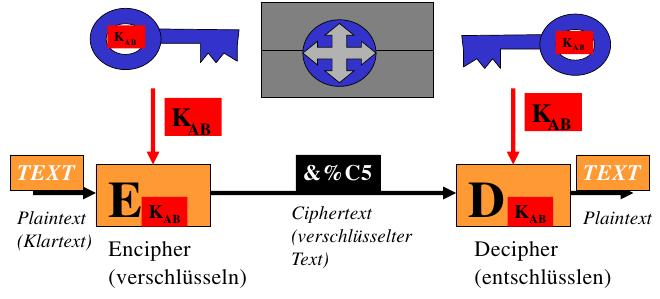
\includegraphics[width=\textwidth]{img/V5.1.jpg}
	\caption{Symetric (secret) Key System}
	\label{}
\end{figure}

\sse{Schlüsselverteilung}
\begin{figure}[H]
	\centering
	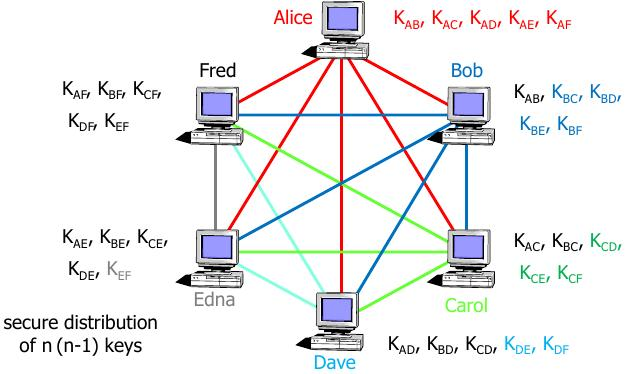
\includegraphics[width=\textwidth]{img/V5.2.jpg}
	\caption{Secure Distribution of n(n-1) keys}
	\label{}
\end{figure}
\ul
	\li Bei nur Zwei Kommunikationspartnern braucht es nur einen Schlüssel
	\li Bei mehreren Kommunikationspartnern braucht es für jedes Kommunikationspaar einen Schlüssel.
	\li In einem Netz mit n Teilnehmer benötigt jeder n-1 Schlüssel
	\li Weil jeweils 2 Schlüssel gleich sind ist die Totale Anzahl benötigter unterschiedlicher Schlüssel $\frac{n*(n-1)}{2}$
\ulE

\se{Asymetrische Schlüssel Systeme}
\definition{Asymetrische Verfahren}{Zum Ver- und Entwschlüsseln werden unterschiedliche Schlüssel verwendet}
\begin{figure}[H]
	\centering
	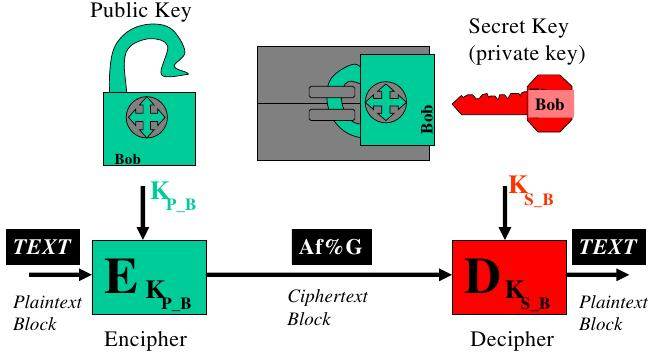
\includegraphics[width=\textwidth]{img/V5.3.jpg}
	\caption{Public Key Systems}
	\label{}
\end{figure}
\ul
	\li Sender und Empfänger verwenden unterschiedliche Verfahren
	\li Verschlüsselt wird mit einem öffentlichen Schlüssel
	\li Entschlüsselt wird mit einem geheimen Schlüssel
	\li Die Anzahl Schlüssel wächst linear mit der Anzahl Teilnehmer
\ulE
\examp{Asymetrische Verschlüsselung}{Wer Bob eine verschlüsselte Meldung senden will, besorgt sich Bob‘s öffentlichen
Schlüssel und verschlüsselt die Meldung mit diesem Schlüssel. Man geht davon aus,
dass Bob der einzige ist, der den passenden geheimen Schlüssel hat und damit die
Meldung wieder entschlüsseln kann.}
\sse{Verfahren}
\dl
	\di{Rivest-Shamir-Adleman(RSA)} basiert auf der Idee, dass die Faktorisierung einer grossen Zahl eine sehr Aufwändige Angelegenheit ist, das erzeugen einer grossen Zahl durch Primzahlenmultiplikation jedoch trivial.
	\di{Elliptic-Cuve-Cryptography (ECC)} basiert darauf, dass es sehr aufwendig ist, diskrete Logarithmen auf elliptischen ruven zu berechnen. Bietet bereits bei kurzen Schlüssellängen ein hohes Mass an Sicherheit. Bsp. WAP
	\di{Eigamal-Kryptosystem} beruht auf dem mathematischen Problem des diskreten Logarithmus.
	\di{Rabin-Kryptosystem} basiert auf einem Faktorisierungsproblem, ist mit RSA verwandt. Wir wegen bestimmten Angriffsmöglichkeiten kaum verwendet.
\dlE

\se{Symetrische Verfahren vs. Asymetrische}
\ul
	\li Symetrische sind weniger rechenintensiv, ermöglicht verschlüsselung von GBit/s Datenströmen
	\li Symetrische erfordern den sicheren Austausch des Schlüssels
	\li Auf Embeded Systemen ist die Rechenleistung zu gering für komplizierte Verschlüsselungsverfahren. Bsp. RFID Chip
\ulE

\se{Hybrid Verschlüsselungsverfahren}
\definition{Hybridverfahren}{Hybride Kryptosysteme verwenden Public Key Verfahren für den Austausch der
geheimen symmetrischen Schlüssel und Symmetric Key Verfahren für die eigentliche
Meldungsverschlüsselung.}
\examp{Hybridverfahren}{TLS, Transport Layer Security/SSL, Secure Socket Layer}

\se{Stream Cipher System}
\definition{Stromchiffre}{Die kleinsten darstellbaren Klartexteinheiten (Bit, Byte, Zeichen, Wort) werden sukzessiv mit einem Cipherstream verknüpft.}
\ul
	\li Der Cipherstream wird normalerweise mit einem Schlüsselgenerator produziert
	\li Der Schlüsselgenerator liefert anhand eines geheimen Keys unterschiedliche (pseudo) Zufallsfolgen
	\li Jedes Bit wird mit einem Bit des Schlüsselstroms XOR verknüpft
	\li Entschlüsselt wird, indem jedes Bit erneut XOR mit dem Schlüsselstrom verknüpft wird
	\li Es dürfen keine Bits verloren gehen und die Schlüsselgeneratoren müssen synchron arbeiten
\ulE

\sse{WEP}
\ul
	\li Der Pseudo Random Stream wird für jedes Paket neu gestartet, um bei verloren gegangenen Pakteten nicht aus dem Takt zu geraten
	\li Der für jedes Paket verwendete Schlüssel besteht aus  einem offenen übertragenen Teil und einem geheimen Schlüssel
	\li Der offenen Teil sorgt dafür, dass jedes Paket mit einer andern Zahlenfolge verschlüsselt wird
	\li Falls sich der Initialvektor wiederholt, werden zwei Pakete mit derselben Schlüsselsequenz verschlüsselt
	\li Da die Klartexte bzw. gewisse Paketteile wie IP Version, Protocol type bekannt sind, können die Bytes des Schlüssels erraten werden
\ulE

\se{Block Cipher System}
\ul
	\li Typische Blockgrössen sind 64, 128, 192, 256 Bit
	\li zu kurze Blöcke werden aufgefüllt, zu lange fragmentiert.
	\li Beispiele: DES, Camellia, RC2, AES, ...
\ulE
\begin{figure}[H]
	\centering
	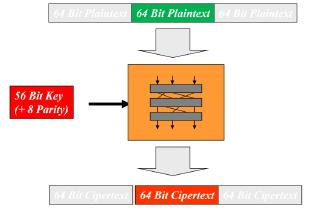
\includegraphics[width=\textwidth]{img/V5.4.jpg}
	\caption{Block Cipher Principle}
	\label{}
\end{figure}

\sse{Cipher Block Chaining CBC}
\expl{CBC}{Jeder Block wird XOR mit einem Chifferblock verknüpft. Jeder chiffertext Block basiert auf den vorhergegangnen Plain Text blocks. Für den ersten Block wird ein Initialisierungsvektor verwendet.}

\sse{Block Cipher Counter CTR}
\expl{CTR}{Überführt einen Block in einen Chifferstream. Generiert den nächsten Schlüsselstream block durch fortlaufender verschlüsselung mit einem Zählerschlüssel.}

\sse{Cipher Feedback CFB}
\expl{CFB}{In diesem Modus wird, wie in der Abbildung dargestellt, die Ausgabe der Blockchiffre mit dem Klartext bitweise XOR (exklusives ODER) verknüpft um daraus den Geheimtext zu bilden. Diese Betriebsart bzw. dieser Modus ergibt damit eine Stromchiffre. Die ausgegebenen Geheimtextdaten fließen als Eingabe in den nächsten Block zur Verschlüsselung.}

\sse{Feistel Blockciphers}
\expl{Feistelchiffre}{Allgemeine Struktur, mit der Blockchiffren realisiert werden können.}

\sse{Des Algorithmus}
\expl{Data Encription Standard}{Auf den 64 Bit Block wird eine initiale Permutation angewandt. Danach wird der Block in
zwei Teile aufgeteilt und jeder Teil in ein 32 Bit Register gespeichert. Die beiden
Blockhälften werden in Folge als linke und rechte Hälfte bezeichnet. Auf die rechte
Blockhälfte wird die Feistel-Funktion angewandt. Danach wird die rechte Hälfte mit der
linken Hälfte XOR verknüpft und das Ergebnis im Register der nächsten Runde für die
rechte Hälfte gespeichert. In das linke Register der nächsten Runde wird die
ursprüngliche rechte Blockhälfte kopiert. Nach Ende der letzten Runde werden die
beiden Hälften wieder zusammengeführt und eine finale Permutation durchgeführt. Dabei
handelt es sich um die inverse Permutation zur initialen Permutation.
Die Entschlüsselung wird mit dem gleichen Algorithmus durchgeführt, wobei die
einzelnen Rundenschlüssel in umgekehrter Reihenfolge verwendet werden.}

\sse{3DES}
\expl{3DES}{Bei 3DES wird jeder Datenblock mit einem DES-Schlüssel K1 chiffriert, dann mit K2
dechiffriert und mit K3 chiffriert. Dieses Verfahren wird auch als EDE (Encrypt-Decrypt-
Encrypt) bezeichnet.
Die Schlüssellänge von 3DES ist mit 168 Bits dreimal so groß wie bei DES (56 Bits),
wodurch die Schlüsselkomplexität auf den ersten Blick um den Faktor 2\^112 gesteigert
wird. Die effektive Schlüssellänge liegt allerdings nur bei 112 Bits, bedingt durch die
Möglichkeit der sog. meet in the middle attack. 3DES wird mittlerweile als ähnlich sicher
wie moderne Verschlüsselungsverfahren mit 128 Bits Schlüssellänge angesehen. 3DES
ist aber relativ langsam, da der Rechenaufwand durch die dreimalige Verschlüsselung
hoch ist. Man beachte im Übrigen, dass es mehrere Methoden gibt, DES dreimal
anzuwenden, Tuchmans 3DES ist nur eine davon.}
\definition{Meet in the middle Angriff}{Besitzt der Angreifer ein Paar aus Klartext und Chiffre, so kann er die Verschlüsselung von beiden Seiten angreifen. Er verschlüsselt den Klartext mit sämtlichen möglichen Schlüssel für Stufe1 und verschlüsselt die so entstandenen Texte ebenfalls mit allen möglichen Schlüsseln für Stufe 2. Dies vergleicht er mit den Ergebnissen der Entschlüsselung des Chiffretextes sämtlicher Schlüssel. Dadurch wird die Anzahl Möglichkeiten drastisch gesenkt und eine Brut Force Attacke wird realistischer.}

\sse{Advanced Encryption Standard AES}
\expl{AES}{Der Rijndael-Algorithmus besitzt eine variable Blockgröße von 128, 192 oder 256 Bit und eine variable Schlüssellänge von 128, 192 oder 256 Bit. Rijndael bietet ein sehr hohes Maß an Sicherheit; erst mehr als 10 Jahre nach seiner Standardisierung wurde der erste, theoretisch interessante, praktisch aber nicht relevante Angriff gefunden. AES schränkt die Blocklänge auf 128 Bit ein, während die Wahl der Schlüssellänge von 128, 192 oder 256 Bits unverändert übernommen worden ist.}

\se{Public and secret Keys}
\begin{figure}[H]
	\centering
	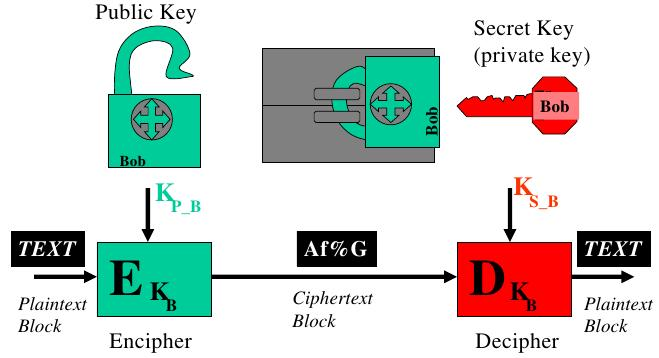
\includegraphics[width=\textwidth]{img/V5.5.jpg}
	\caption{Public and Secret Key}
	\label{}
\end{figure}
\expl{Funktionsweise}{Möchte der Absender dem Empfänger etwas schicken, so besorgt er sich dessen Public Key und verschlüsselt die Nachricht. Nur der Empfänger kann die Nachricht entschlüsseln, weil nur er den private Key besitzt.}
\expl{öffentliche Schlüsselsysteme}{Basieren auf "Einweg-Funktionen", die nicht umkehrbar sind. Z.B: Modulo oder die Multiplikation zwei grosser Primzahlen (Primfaktorzerlegung ist schwierig).}

\se{RSA}
\begin{figure}[H]
	\centering
	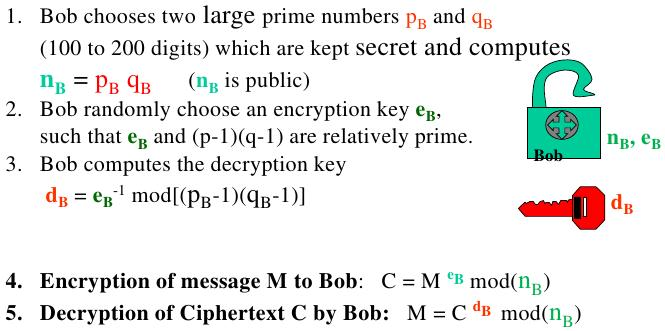
\includegraphics[width=\textwidth]{img/V5.6.jpg}
	\caption{RSA}
	\label{}
\end{figure}


\sse{Schlüsselerzeugung}
\ul
	\li  Wähle zwei grosse Primzahlen p und q (In der Praxis werden diese Primzahlen durch
	Wählen einer Zufallszahl und darauf folgendes Anwenden eines Primzahltests
ermittelt. http://de.wikipedia.org/wiki/Primzahltest)
 \li Berechne n = p.q
 \li Wähle eine kleine Zahl e mit ggT(e, j(n)) = 1, wobei j(n) = (p-1)(q-1) Beachte:
j(n)=Eulerfunktion von n = Anzahl der natürlichen Zahlen zwischen 1 und n, welche zu
n teilerfremd sind
 \li Berechne d mit d.e=1 mod j(n) mit Hilfe des erweiterten Euklidischen Algorithmus
 \li Halte d als geheimen Schlüssel und gib (e, n) als öffentlichen Schlüssel bekannt
\ulE

\sse{Ver- und Entschlüsseln der Nachricht}
\ul
	\li  Verschlüsselte Nachricht:
 c = me mod n
 	\li Entschlüsselung:
 m = cd mod n

\ulE

\expl{RSA}{Im Gegensatz zu einem symmetrischen Schlüssel ist ein RSA-Schlüssel keine reine
Zufallsfolge von Bits, sondern das Produkt von zwei (zufällig) gewählten grossen
Primzahlen. Daher sind bei k-Bit Schlüssellänge bei den asymmetrischen Schlüsseln
nicht alle 2\^k Kombinationen möglich, wie dies bei symmetrischen Schlüsseln der Fall
ist.
}

\se{ECC}
\expl{ECC}{basiert darauf, dass es sehr aufwendig ist, diskrete Logarithmen auf elliptischen Bahnen zu berechnen. Bietet bei kurzen Schlüssellängen ein hohes Mass an Sicherheit.}
\examp{ECC}{WAP}


\se{Diffie Hellmann}
\definition{Diffie Hellmann Verfahren}{Ermöglicht es, über einen unsicheren Kanal geheime Botschaften zu übertragen.}
\begin{figure}[H]
	\centering
	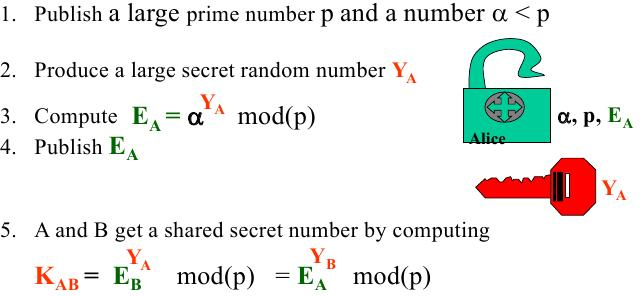
\includegraphics[width=\textwidth]{img/V6.1.jpg}
	\caption{DH}
	\label{}
\end{figure}
\ul
	\li 
Alice und Bob einigen sich über einen öffentlichen Kanal auf eine Primzahl p und eine Zahl g. Alice denkt sich jetzt eine Zahl a < p aus, die sie geheim hält. Ebenso denkt sich Bob eine Zahl b < p aus, die auch er geheim hält. 
\li Alice berechnet jetzt die Zahl

ka = ga(mod p)

und schickt diese Bob. Bob berechnet analog die Zahl

kb = gb(mod p)

und schickt diese Alice. 
\li Das gemeinsame Geheimnis K berechnet Alice jetzt aus ihrer geheimen Zahl a und der Zahl kb von Bob mit

K = kba (mod p).

Die gleiche Zahl kann Bob analog mit

K = kab (mod p)

berechnen.

\li 
Das Geheimnis K kann jetzt von beiden Seiten als Schlüssel für eine symmetrische Verschlüsselung verwendet werden. 
\li Die passive Angreiferin Eve, die die Kommunikation zwischen Alice und Bob abhört, kennt nur die Zahlen p, g, ka und kb, nicht jedoch a oder b. Ohne diese ist es ihr nur möglich, K zu berechnen, wenn sie

ka = ga (mod p), also a = logg(ka) (mod p)

lösen kann. Für große Zahlen p, a und b kann dies aber mit heutiger Rechenkapazität Jahrhunderte oder länger dauern.
\ulE


\se{Verschlüsselungssysteme Knacken}
\definition{Sicherheit}{Die Sicherheit nimmt mit der Schlüssellänge exponentiell zu, weil die Schlüsselvielfalt exponentiell wächst.}

\expl{Schlüssellänge}{Asymetische Schlüssel müssen länger sein als vergleichbare symetrische, weil nur die in der Zahl vorkommenden Primzahlen verwendet werden.}

\se{Digitale Signaturen}
\definition{Signaturen}{Gewährleisten der Integrität, Authentizität}

\sse{Hash}
\definition{Hash}{Bildet Nachricht auf k-Bit Hash ab}

\sse{MD5}
\expl{MD5}{Block wird gehased, mit nächstem Block verküpft, gehased, ...}
\begin{figure}[H]
	\centering
	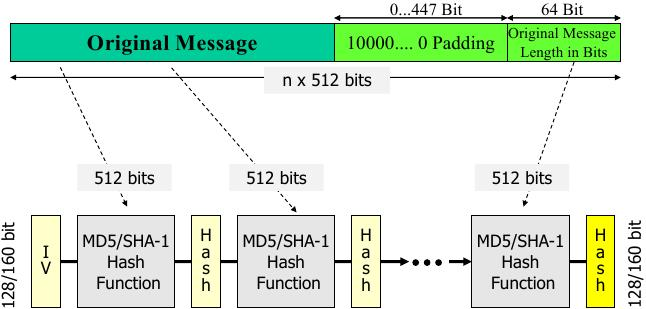
\includegraphics[width=\textwidth]{img/V6.2.jpg}
	\label{}
\end{figure}
\begin{figure}[H]
	\centering
	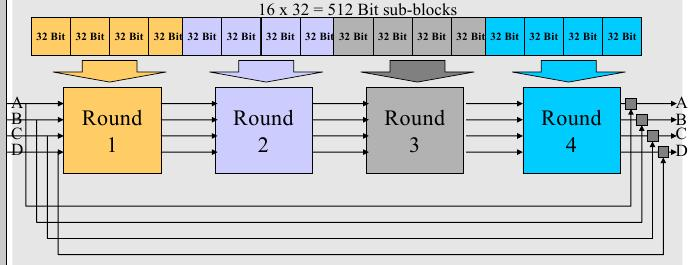
\includegraphics[width=\textwidth]{img/V6.3.jpg}
	\label{}
\end{figure}
\begin{figure}[H]
	\centering
	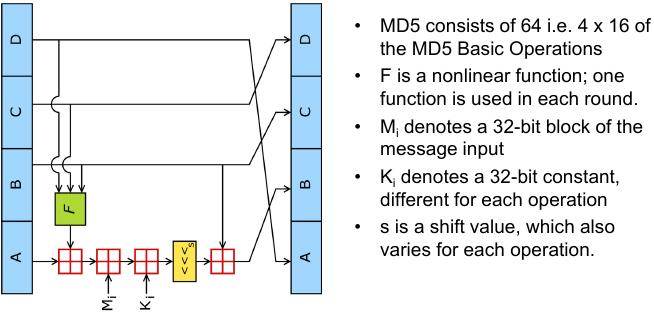
\includegraphics[width=\textwidth]{img/V6.4.jpg}
	\label{}
\end{figure}
\ul
	\li Es darf nicht vom Hash auf den Key geschlossen werden können
	\li Es sollten keine Meldungen auftreten, die den gleichen Hash erzeugen
\ulE
\begin{figure}[H]
	\centering
	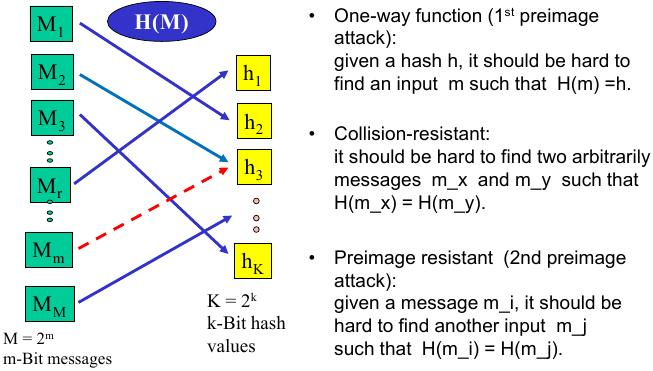
\includegraphics[width=\textwidth]{img/V6.5.jpg}
	\label{}
\end{figure}

\sse{Keyed Hash}
Schlüssel wird noch symetrisch verschlüsselt, daher kann er nur vom Absender kommen.
\begin{figure}[H]
	\centering
	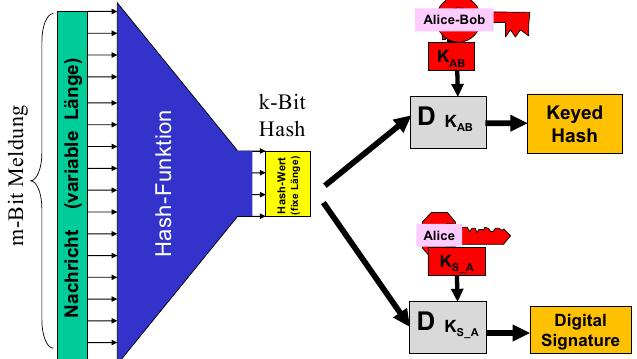
\includegraphics[width=\textwidth]{img/V6.6.jpg}
	\label{}
\end{figure}

\sse{Asymetrisch Keyed Hash}
\ol
	\li A erhält Schloss von irgendjemandem. 
	\li Lässt Schloss von Empfänger öffnen um sicher zu gehen, dass das Schloss das richtige ist.
\olE

\sse{Message Authentication Codes based on Keyed One-Way Hash}
\begin{figure}[H]
	\centering
	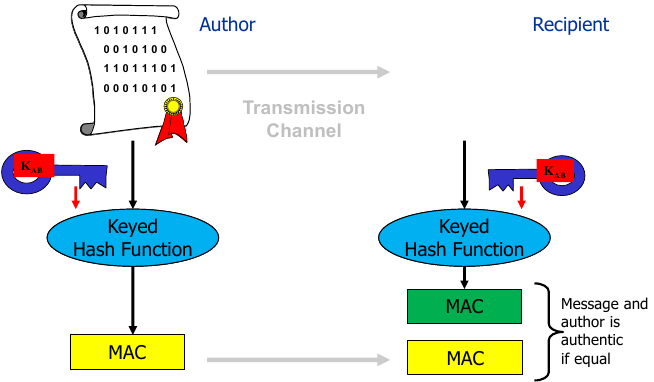
\includegraphics[width=\textwidth]{img/V6.7.jpg}
	\label{}
\end{figure}

\sse{DSS}
\begin{figure}[H]
	\centering
	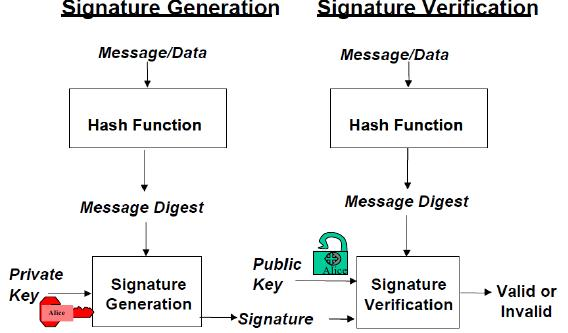
\includegraphics[width=\textwidth]{img/V6.8.jpg}
	\label{}
\end{figure}
\begin{figure}[H]
	\centering
	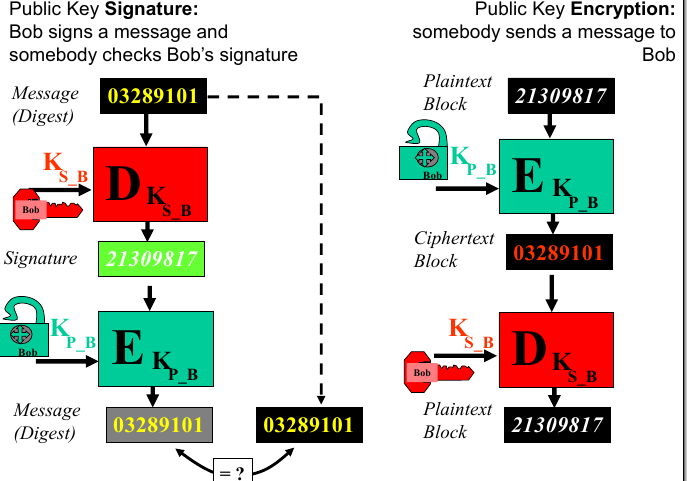
\includegraphics[width=\textwidth]{img/V6.9.jpg}
	\caption{DSS Beispiel}
	\label{}
\end{figure}


\se{Digitale Signaturen}
\definition{Digitale Signatur}{Echtheitserklärung}
\examp{Einfache, allgemeine elektronische Signatur}{Name unter einer E-Mail}
\examp{fortgeschrittene elektronische Signatur}{Unterschrift unter einer E-Mail, welche mit dem einer
Person zugeordneten Private/Public Key (Zertifikat) produziert wurde. Ermöglicht Überprüfung von Authentizität und Integrität der E-Mail.}
\examp{qualifizierte elektronische Signatur}{Unterschrift, welche die per Gesetz geforderte Unterschrift
ersetzt. Basiert auf einem „qualifizierten digitalen Zertifikat“. (z.B. Post SuisseID)}

\sse{Wünschbare Eigenschaften}
\ul
	\li Fälschungssicherheit (Dokument kann nicht mehr verändert werden)
	\li Authentizität (Zweifelsfreie Zuordnung zu einer best. Person)
	\li Unleugbarkeit (Beweist, dass der Unterzeichner das Dokument studiert/erstellt hat)
	\li Willenserklärend (Dokument kann nur willentlich unterschrieben werden)
\ulE

\sse{Zertifikatausgabestellen CH}
\begin{figure}[H]
	\centering
	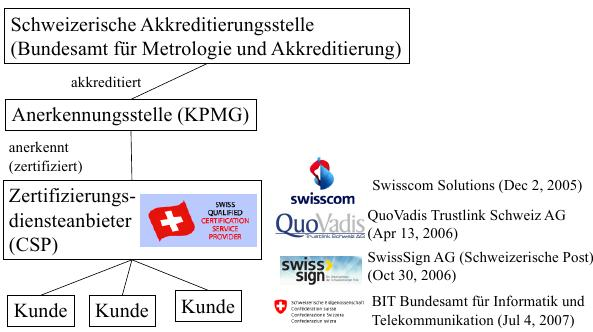
\includegraphics[width=\textwidth]{img/V7.1.jpg}
	\caption{}
	\label{}
\end{figure}

\dl
	\di{Handunterschrift}: \\
		\ul
			\li +einfach herzustellen
			\li +einfach zu fälschen
			\li -einfach per Kopie übertragbar
			\li +Rechtslage: Andere Partei muss beweisen, dass sie etw. nicht unterschrieben haben
		\ulE
	\di{Digitale Unterschrift}: \\
		\ul
			\li -komplex Generierungsprozess
			\li + abs. überprüfbar
			\li + kein Bit kann unerkannt geändert werden
			\li - Rechtslage: Sie müssen beweisen, dass Sie etw. nicht unterschr. haben
		\ulE
\dlE


\ch{Zertifikate}
\expl{Man in the middle Attack}{Angreifer schickt Client einen Link. Der User landet nicht bei der Bank sondern beim Angreifer und dieser schiebt einem ein eigenes Schloss unter. Anschliessend holt er sich das Schloss der Bank und hängt somit in der Mitte.}
\definition{Zertifikat}{Schloss muss zertifiziert sein, damit Client Herkunft verifizieren kann.}
\begin{figure}[H]
	\centering
	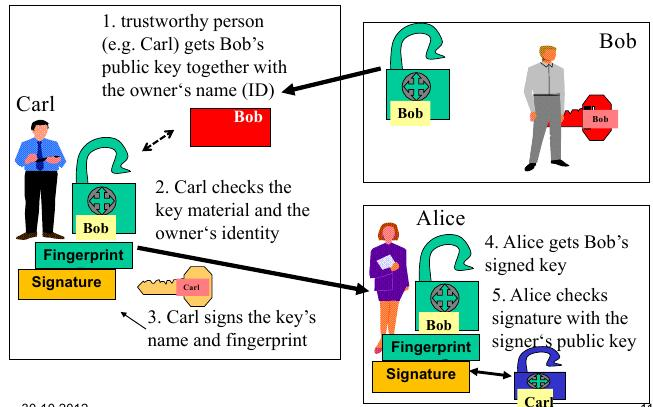
\includegraphics[width=\textwidth]{img/V7.2.jpg}
	\caption{Jemand verifiziert den Schlüsselbesitzer und signiert den Schlüssel}
	\label{}
\end{figure}

\begin{figure}[H]
	\centering
	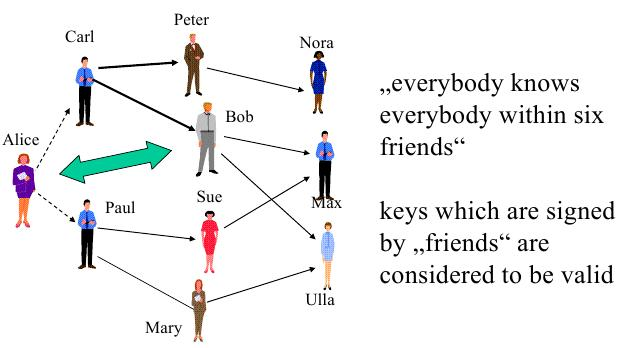
\includegraphics[width=\textwidth]{img/V7.3.jpg}
	\caption{Web of Trust: Jemand verifiziert den Besitzer und signiert den Schlüssel}
	\label{}
\end{figure}

\se{Public Key Infrastructure}
\begin{figure}[H]
	\centering
	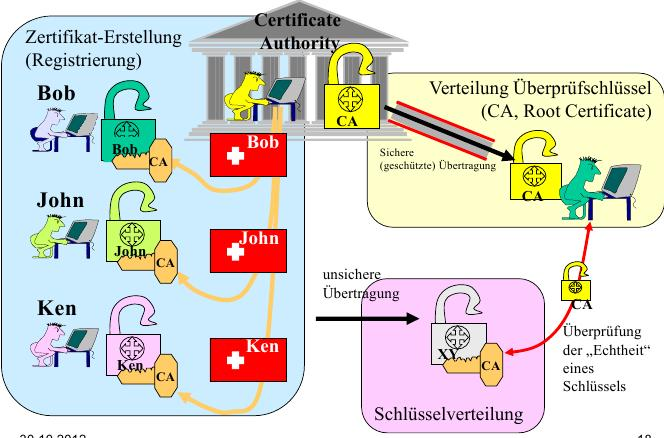
\includegraphics[width=\textwidth]{img/V7.4.jpg}
	\caption{PKI}
	\label{}
\end{figure}

\ul
	\li Zertifikate werde von Zertifizierungsstelle generiert
	\li Zertifikate müssen über sicheren Kanal zum Client gelangen
\ulE

\ch{Zertifikatklassen}
\dl
	\di{Class 0} Demo certificates for testing. No authentication whatever required.
Usually expire after 30 days.
	\di{Class 1} Ascertain that a given e-mail address exists and that the owner of the respective
public key has access to it. Low-level identity check.
	\di{Class 2} Designed for companies and thus a personal identification is not necessary. A copy
of proof of the register of companies to establish persons authorised to sign and a
written request will suffice.
	\di{Class 3} Apart from the verification of the e-mail address also a personal identification of a
person on the basis of an ID or passport required.
For companies, personal presence of authorized person required.
	\di{Class 4} Identification process must take place at the site of an official registration
authority (state or community office)
\dlE

\begin{figure}[H]
	\centering
	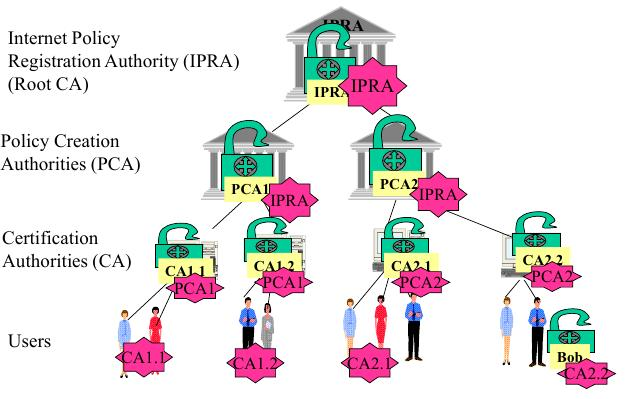
\includegraphics[width=\textwidth]{img/V7.5.jpg}
	\caption{Hirarchisches Vertrauen}
	\label{}
\end{figure}


\ul
	\li Zertifikate landen durch Patches im Browser
\ulE
\begin{figure}[H]
	\centering
	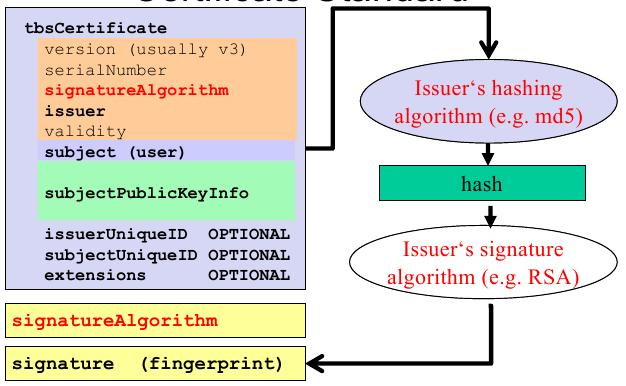
\includegraphics[width=0.75\textwidth]{img/V7.6.jpg}
	\caption{ITU-.509 (ISO/IEC 9594-8) Certificate Standard}
	\label{}
\end{figure}

\begin{figure}[H]
	\centering
	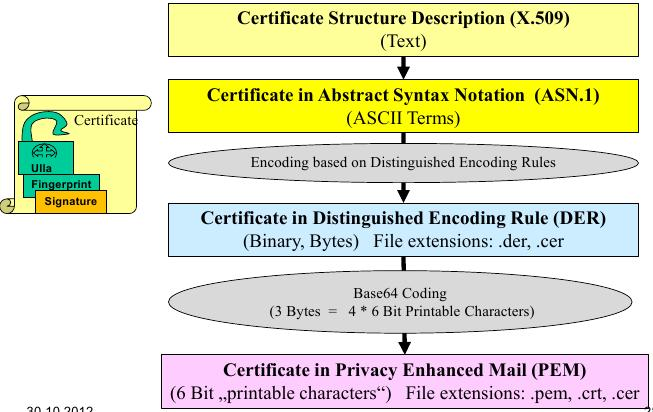
\includegraphics[width=0.75\textwidth]{img/V7.7.jpg}
	\caption{X.509 (ISO/IEC 9594-8) Certificate Formats}
	\label{}
\end{figure}

\sse{Key usage Extension}
\begin{figure}[H]
	\centering
	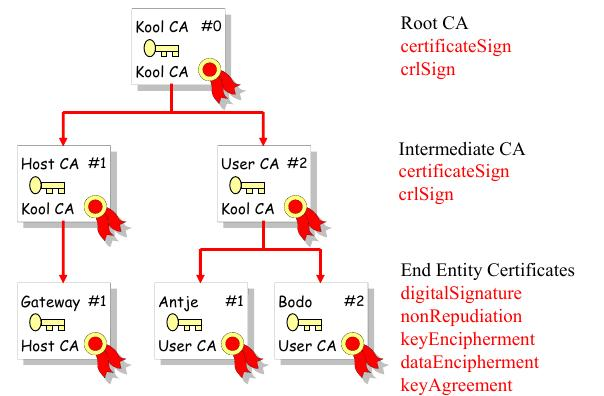
\includegraphics[width=0.75\textwidth]{img/V7.8.jpg}
	\caption{Key usage extension}
	\label{}
\end{figure}

\sse{Path length constraint}
\begin{figure}[H]
	\centering
	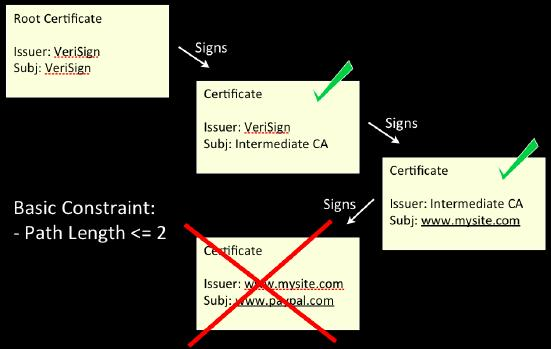
\includegraphics[width=0.75\textwidth]{img/V7.9.jpg}
	\caption{}
	\label{}
\end{figure}
\begin{figure}[H]
	\centering
	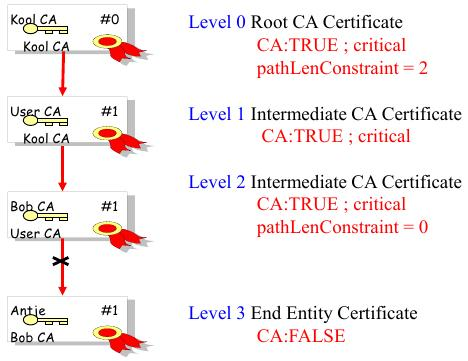
\includegraphics[width=0.75\textwidth]{img/V7.10.jpg}
	\caption{basic constraints - path length constraint}
	\label{}
\end{figure}
\begin{figure}[H]
	\centering
	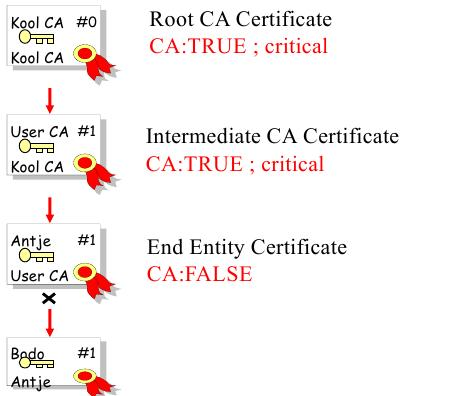
\includegraphics[width=0.75\textwidth]{img/V7.11.jpg}
	\caption{basic constraint - ca flag}
	\label{}
\end{figure}


\ch{Secure Email}
\examp{Verschlüsselte E-mail}{Gegen Industriespionage und zum Datenschutz}
\examp{Signierte E-mail}{Gegen Spam und Phishing}

\se{S/MIME}
\expl{MIME}{Zum Übertragen von Binary Daten mit E-mail}

\ul
	\li Teile der E-mail werden mit boundaries getrennt.
	\li Für jeden Teli wird Codierung und Mime Type angegeben.
	\li Bei Verschlüsselung wird die Signatur in ein eigenes Boundary gepackt.
\ulE

\begin{figure}[H]
	\centering
	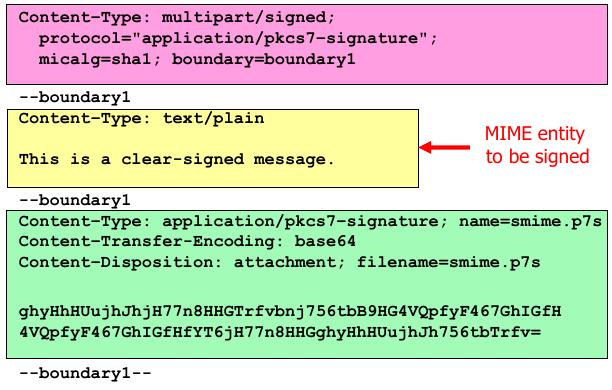
\includegraphics[width=0.75\textwidth]{img/V8.1.jpg}
	\caption{PKCS \# 7}
	\label{}
\end{figure}

\sse{Multipart E-mails}
\ul
	\li Server ändern manchmal Codierung \ra Hash falsch
	\li Provider zerlegen E-mail und analysieren Attachments \ra bauen anschliessend Header in falscher Reihenfolge wieder zusammen
\ulE

\sse{PKCS \#7}
\begin{figure}[H]
	\centering
	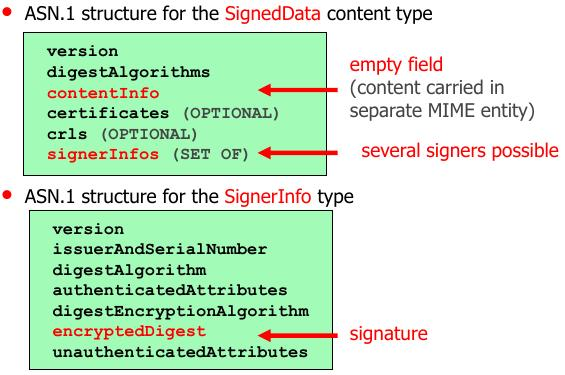
\includegraphics[width=0.75\textwidth]{img/V8.2.jpg}
	\caption{PKCS \# 7}
	\label{}
\end{figure}

\sse{E-mail Verschlüsselung}
\ul
	\li Mailinhalt inklusive Attachments wird verschlüsselt
	\li Header inkl. Betreff wird nicht verschlüsselt
	\li Wichtig ist, dass die Sicherungskopie im Ordner gesendete Mails verschlüsselt ist und ich selbst als Empfänger eingetragen bin, damit ich es wieder entschlüsseln kann.
\ulE

\begin{figure}[H]
	\centering
	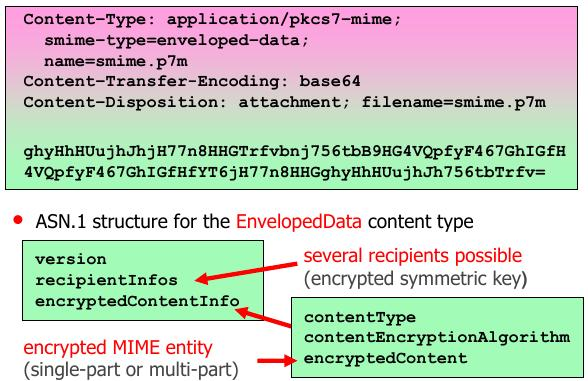
\includegraphics[width=0.75\textwidth]{img/V8.3.jpg}
	\caption{Verschlüsselte E-mail}
	\label{}
\end{figure}

\begin{figure}[H]
	\centering
	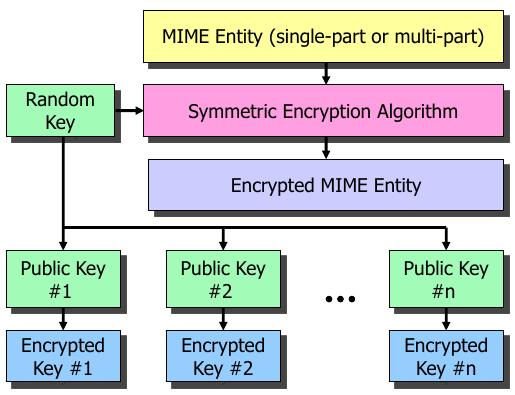
\includegraphics[width=0.75\textwidth]{img/V8.4.jpg}
	\caption{Hybridverschlüsselung bei E-mail}
	\label{}
\end{figure}
\ul
	\li Der symetrische key wird asymetrisch verschlüsselt und in die E-mail eingefügt
	\li Die Nachricht ist symetrisch verschlüsselt
	\li Zwei Möglichkeiten:
		\ul
			\li Zuerst signieren, im zweiten Schritt verschlüsseln
				\ul
					\li Vorteil: Nur binärer Blobb, der verschlüsselt ist (anonyme E-mail)
				\ulE
			\li Zuerst verschlüsseln, dann Hash über das Ganze und signieren
				\ul
					\li Vorteil: Bevor ich etwas entschlüssle, kann ich die Signatur verifizieren
				\ulE
		\ulE
\ulE

\begin{figure}[H]
	\centering
	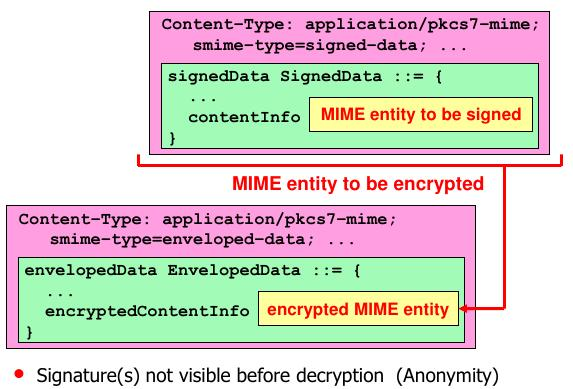
\includegraphics[width=0.75\textwidth]{img/V8.5.jpg}
	\caption{Signing bevor Encryption}
	\label{}
\end{figure}

\begin{figure}[H]
	\centering
	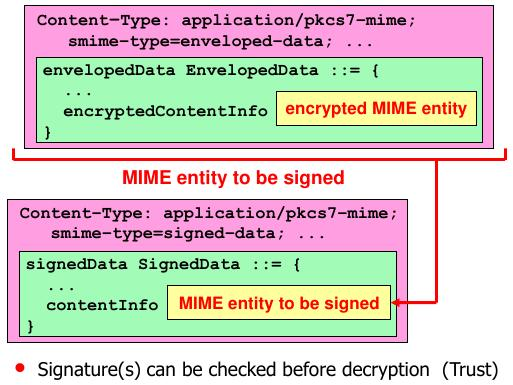
\includegraphics[width=0.75\textwidth]{img/V8.6.jpg}
	\caption{Encryption befor signing}
	\label{}
\end{figure}

\se{Zusammenfassung}
\begin{figure}[H]
	\centering
	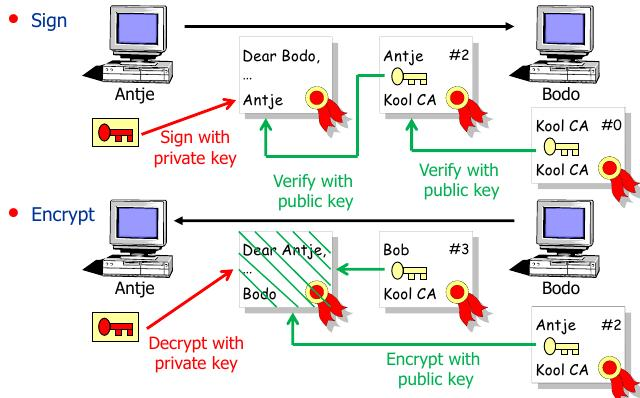
\includegraphics[width=0.75\textwidth]{img/V8.7.jpg}
	\caption{Signing and Encrypting}
	\label{}
\end{figure}

\sse{Signatur}
\ul
	\li A signiert gesammte mail inkl. Attachments mit private key
	\li Zertifikat wird mitgesendet (im PKCS7 Payload)
	\li B braucht CA um Zertifikat zu überprüfen
	\li B überptüft Signatur mit Public Key
\ulE

\sse{Verschlüsselung}
\ul
	\li B verschlüsselt Nachricht symetrisch
	\li B verschlüsselt symetrischen Key asymetrisch mit dem Publiy Key von A
	\li A entschlüsselt den Key mit ihrem private Key und entschlüsselt dann die Nachricht
	\li A überprüft Zertifikat von B
\ulE

\sse{PKCS\#12 Container}

\dl
	\di{Public Key}:\\
	   	\ul
    		\li pk(e,n) 
    		\li PKCS\#1 
    		\li .pem, .dem
    	\ulE
    \di{Private Key}:\\
    	\ul
    		\li pk(d,n,p,q,...) 
    		\li PKCS\#1, PKCS\#9 
    		\li .pem, .dem 
    		\li optional Passwort
    	\ulE
    \di{Zertifikat}:\\
    	\ul
    		\li X.509: 
    		\li Subject+Public Key (Zusammengehörigkeit wird vom CA durch Signatur garantiert) 
    		\li .pem, .dem, .cer, .cert
    	\ulE
\dlE

\begin{tikzpicture}
  \path[mindmap,concept color=brown,text=black]
    node[concept] {PKCS\#12 \\Container \\.ps12}[clockwise from=-25]
    	child[concept color=orange,text=black] { node[concept] {Public Key \\ .pem} }
    	child[concept color=orange,text=black] { node[concept] {Private Key \\ .pem} } 
    	child[concept color=orange,text=black] { node[concept] {Zertifikat \\ .der} };
\end{tikzpicture}

\se{Probleme}
\ul
	\li Wenn Key abläuft, verfallen Signaturen oder E-mails sind nicht mehr lesbar \ra Schlüssel und Zertifikate müssen lokal gespeichert werden
\ulE


\ch{Transport Layer Security TLS}
\expl{SSL/TLS}{TLS war früher SSL}

\begin{figure}[H]
	\centering
	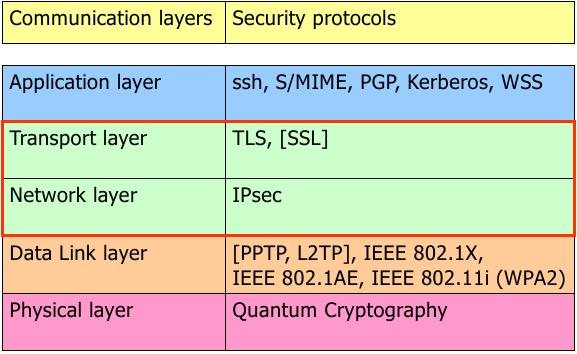
\includegraphics[width=0.75\textwidth]{img/V9.1.jpg}
	\caption{Secure Network Protocols for the OSI Stack}
	\label{}
\end{figure}

\begin{figure}[H]
	\centering
	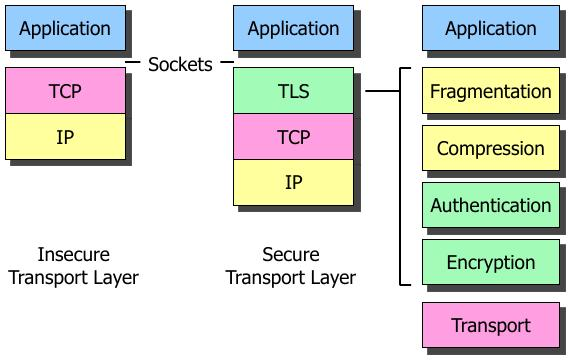
\includegraphics[width=0.75\textwidth]{img/V9.2.jpg}
	\caption{TLS/SSL Protocol Layers}
	\label{}
\end{figure}

\ul
	\li SSL läuft im User Mode
	\li Secure Socket statt normalen socket
\ulE

\se{TLS Record Protocol}
\begin{figure}[H]
	\centering
	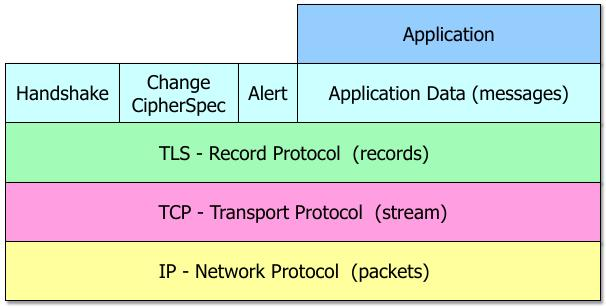
\includegraphics[width=0.75\textwidth]{img/V9.3.jpg}
	\caption{TLS Record Protocol}
	\label{}
\end{figure}

\ul
	\li Fehlersignalisation geht über Alert
	\li TLS Nimmt Block von max. 16'384 Bytes, komprimiert es optional, fügt MAC und Padding hinzu um auf AES Blockgrösse zu kommen.
	\li Ganzer Block wird verschlüsselt
	\li Ablauf:
		\ol
			\li	Fragmentierung
			\li	Kompression
			\li	Authentifikation
			\li	Blockbildung
		\olE
\ulE

\begin{figure}[H]
	\centering
	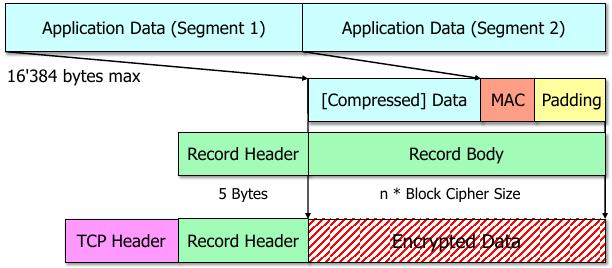
\includegraphics[width=0.75\textwidth]{img/V9.4.jpg}
	\caption{TLS Record Structure}
	\label{}
\end{figure}

\sse{TLS Handshake Protocol}
\begin{figure}[H]
	\centering
	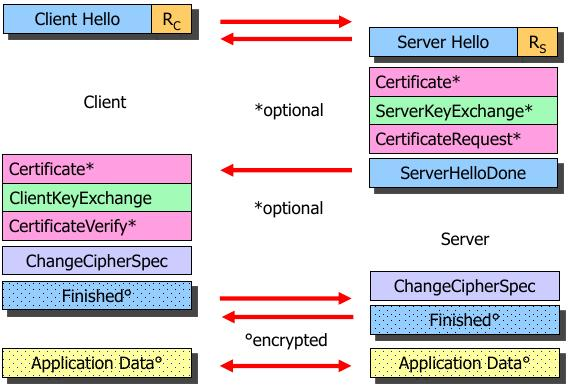
\includegraphics[width=0.75\textwidth]{img/V9.5.jpg}
	\caption{TLS Handshake Protocol}
	\label{}
\end{figure}

\ol
	\li Client beginnt, sendet "Client Hello", sendet NANS (einmahlige Zufallszahl um Replay Attacke zu verhindern)
	\li Server sendet "Server Hello", nimmt meist die erste Cipher Suite des Client angebots, dass für ihn o.k. ist
	\li Jetzt ist Cryptoverfahren klar
	\li Server sendet optional Zertifikat, öffentlicher Key, Aufforderung zu Zertifikat + ServerHelloDone
	\li Wenn Client aufgefordert wird zu clientseitigem Zertifikat \ra sendet Zertifikat
	\li Client sendet Key mit
	\li ChangeCipherSpec: 1Byte Paket welches signalisiert, das auf Cipher umgestellt wird. Die Finished Message testet Verschlüsselung
	\li Server sendet auch changeSipherSpec (verschlüsselte Checksum) und schaltet um. Wenn etwas nicht stimmt, z.B. Hast falsch weil zusätzliche Pakete eingeschleust wurden: sendet Alert.
	\li Server und Client tauschen verschlüsselt Application Data aus.
\olE

\sse{Aufgaben des TLS}
\ul
	\li Endpunktauthentisierung / Identifizierung
	\li Key Establishment (gemeinsamer Schlüssel)
\ulE

\sse{RSA Key Encription}
\ol
	\li Server mit Zertifikat, unterschrieben von CA (z.B: VeriSign)
	\li Wird übertragen an Client
	\li Client besitzt Random Generator (RNG)
	\li Geeriert daraus premasterSecret von 48Byte mit maximaler Entropie
	\li Zufallszahl (pms) wird mit Public Key des Serverzertifikats verschlüsselt
	\li Wird an Server gesendet
	\li Server kann Zufallszahl wieder entschlüsseln
	\li Leitet daraus MasterSecret ab und initialisierungsvektor für CBC ab
	\li Generiert mit diesen Keys die authentisierte Finish-Meldung
\olE
\expl{Sicherheit}{Wenn der Server den Private Key zu seinem Zertifikat hat, kann er das preMasterSecret entschlüsseln und die Finishmeldung senden}

\expl{Gefährlichkeit}{Gefährlich, wenn Authentisierung und Schlüsselgenerierung gekoppelt wird, daher sollte heute RSA Key Encription nicht mehr eingesetzt werden}

\ul
	\li Heute wird authentisierung von der Schlüsselgeneration getrennt
\ulE

\sse{Diffie Hellman Exchange}
\ul
	\li Client und Server generieren Zufallszahl s mit RNG. Dies ist private Key
	\\ Public Key $S = g^s mod p$ (p Primzahl)
	\li Server macht das gleiche \ra c
	\\ \ra Diskreten Logarithmus zum knacken von c und s sehr schwierig
	\li Beide übertragen Public Key und verschlüsseln eweils mit Public Key des andern
	\li PFS: Für jede Session werden mit dem RNG neue Schlüssel generiert\\
	Server hat für jede TLS Verbindung einen andern private Key
	\\ \ra Unterschied zu RSA Key Encription: erzeugt jedesmal einen neuen Weg werf Key
	\li preMasterSecret wird gebildet mit Public Key des Servers \\
	$= S^cmod p = g^sc$
\ulE

\sse{Resuming a TLS session}
\begin{figure}[H]
	\centering
	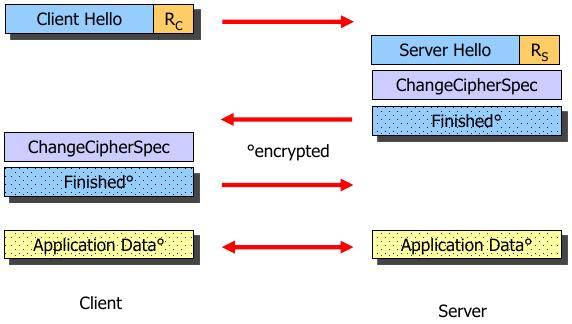
\includegraphics[width=0.75\textwidth]{img/V9.6.jpg}
	\caption{}
	\label{}
\end{figure}

\ul
	\li Für jedes grafische Element einer Webseite wird eigene Http Verbindung aufgemacht \ra Verschlüsselung aufwendig
	\li Server kann Session Kontext Container wieder verwenden \ra leitet von preMasterSecret neuen masterSecret ab
\ulE

\ol
	\li Client sendet Session ID
	\li Server schaut ob er noch Session Container hat und generiert aus preMasterSecret neuen Mastersecret ab
	\li Server sendet Finish
\olE


\se{TLS Schwachstellen}
\ul
	\li Im kryptographischen Umfeld können Fehlermeldungen verhängnisvoll sein. Aufgrund von Fehlermeldungen kann der Schlüssel Stück für Stück erraten werden.
\ulE

\sse{BEAST}
\expl{BEAST}{Browser Exploit Against SSL/TLS}
The exploit uses a known-plaintext attack on the Cipher-Block-Chaining
(CBC) encryption vulnerability of SSL 3.0 and TLS 1.0
which has been known since 2001 and was fixed by TLS 1.1 in 2006.

\sse{CRIME}
\expl{CRIME}{Compression Ratio Info-leak Made Easy}
\ul
	\li Attacke auf den Kompressionsmechanismus
	\li Man-in-the Middle Attacke
	\li Javascript speist vermutetes Cookie Sicherheitswort vor Komprimierung ein. Weil komprimierung mit Lempel-Zif kleineres Paket erzeugt, desto mehr das vermutete Sicherheitswort mit dem effektiven übereinstimmt kann so mit einigen Versuchen das Cookie Secret Wort erraten werden.
	\li Einzige Fix-Möglichkeit: Komprimierung deaktivieren
\ulE


\se{TLS-based Authentication}
\sse{HTTP Basic Access Authentication}
\begin{figure}[H]
	\centering
	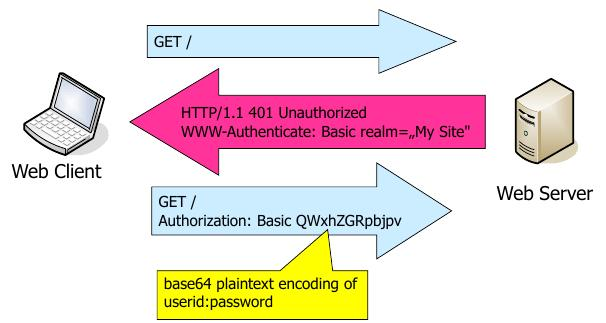
\includegraphics[width=0.75\textwidth]{img/V10.1.jpg}
	\caption{HTTP Basic Access Authentication}
	\label{}
\end{figure}

\ul
	\li Normales Get an geschützen Bereich senden
	\li Fehlermeldung
	\li Aufforderung für Passwort
	\li Passwort wird als Base64 übermittelt: Klartext
\ulE

\sse{HTTP Digest Access Authentication}
\begin{figure}[H]
	\centering
	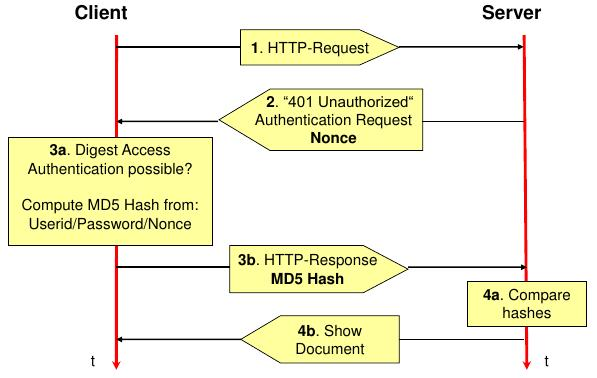
\includegraphics[width=0.75\textwidth]{img/V10.2.jpg}
	\caption{HTTP Digest Access Authentication}
	\label{}
\end{figure}

\ul
	\li Nicht Passwort sondern PoswortHash wird übermittelt
\ulE

\sse{EAP-Based Authentication and Access Control}
\begin{figure}[H]
	\centering
	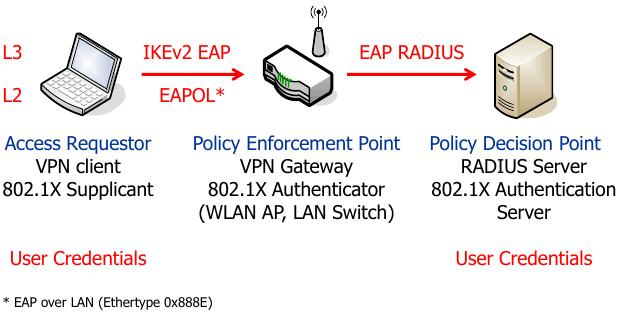
\includegraphics[width=0.75\textwidth]{img/V10.3.jpg}
	\caption{EAP-Based Authentication and Access Control}
	\label{}
\end{figure}

\ul
	\li Client möchte in Netzwerk rein \ra muss sich Authentifizieren
	\li Client hat noch keine IP Adresse
	\li Geht an Switch/Access Point
	\li Authentisierungsserver überprüft Passwort (RADIUS Server schaut in Active Directory nach)
\ulE

\begin{figure}[H]
	\centering
	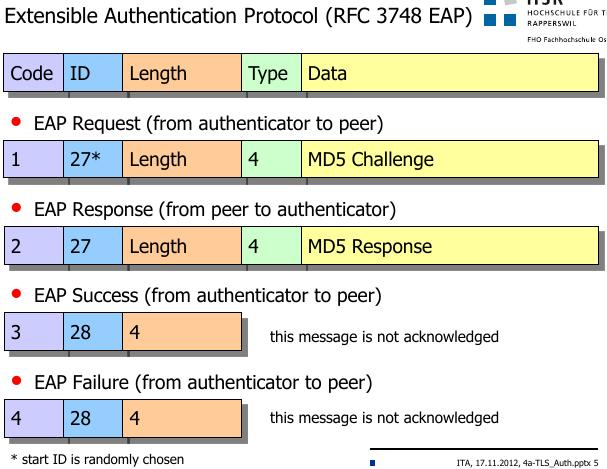
\includegraphics[width=0.75\textwidth]{img/V10.4.jpg}
	\caption{EAP (Extensible Authentication Protocol)}
	\label{}
\end{figure}

\ul
	\li Nicht MD5 und MS Chap verwenden!
\ulE

\sse{EAP-MD5 Authentication protected by EAP-TTLS}
\begin{figure}[H]
	\centering
	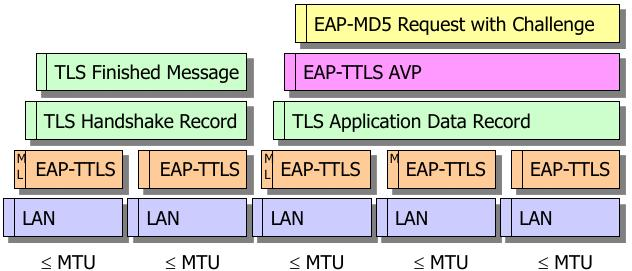
\includegraphics[width=0.75\textwidth]{img/V10.5.jpg}
	\caption{EAP-MD5 Authentication protected by EAP-TTLS}
	\label{}
\end{figure}

\ul
	\li Wenn bei Finish Meldung Zertifikat übetragen wird \ra Paket grösser als max MTU \ra wird fragmentiert
	\li Dann wird umgeschaltet auf TLS Application Data Record
	\li Auc hier wird fragmentiert. Solange noch Pakete kommen, wird das MoreFragments-Flag gesetzt, damit der Empfänger es wieder zusammensetzen kann.
	\li Authentifizierung im WLAN läuft meistens so: Zuerst wird mit TLS End-zu-End verschlüsselt, bevor irgendwelche Passwörter ausgetauscht werden.
	\li EAP-TLS setzt immer Client Authentifizierung auf Basis eines X.509 Zertifikates voraus, wird jedoch nur von Banken etc. eingesetzt
	\li EAP-TTLS: Client authentication based on EAP-MD5, EAP-MSCHAP-V2 or EAP-GTC,
often preceded by EAP-Identity. Optionally followed by EAP-TNC for
Trusted Network Connect.
	\li EAP-PEAP: Nicht verwenden, faul
\ulE










\end{document}